\sisetup{separate-uncertainty=true,detect-weight=true,detect-inline-weight=math}

\section{Experiments and Results}

% \uselengthunit{in}\printlength{\textwidth} = 4.8041 in
% \uselengthunit{mm}\printlength{\textwidth} = 121.99854 mm

We evaluated our method on two publicly available data sets, which allows for
the direct comparison with state-of-the-art methods. In addition, we have used a
very challenging data set containing four different MRI sequences of
relapsing-remitting MS patients from a multi-center MS clinical trial, which
represents the large variability in lesion size, shape, location and intensity
as well as varying contrasts produced by different scanners. The trial data set
was used to carry out a detailed analysis of different CEN architectures using
different combinations of modalities, and we compared against competing
segmentation methods.

\subsection{Data Sets and Pre-processing}

% TODO: How was split determined: all scans of the same patient and scanning
% site were put in the same group

% TODO: Why did I choose Lesion-TOADS?

\paragraph{Proprietary data set}

The data set was collected from 67 different scanning sites using different
1.5\,T and 3\,T scanners for a clinical trial in relapsing-remitting MS, and
consists of 377 T1-weighted (T1w), T2-weighted (T2w), proton density-weighted
(PDw), and FLAIR MRIs from 195 subjects. The image dimensions are
\num{256x256x60} voxels with a voxel size of
\SI{0.936x0.936x3.000}{\milli\metre}. All images were skull-stripped using the
brain extraction tool (BET) \cite{jenkinson2005bet2}, followed by an intensity
normalization to the interval $[0,1]$, and a 6 degree-of-freedom intra-subject
registration. To speed-up the training, all images were cropped to a
\num{164x206x52} voxel region-of-interest with the brain roughly centered. The
ground truth segmentations were produced using an existing semiautomatic 2D
region-growing technique, which has been used successfully in a number of large
MS clinical trials (e.g., \cite{kappos2006long},
\cite{traboulsee2008reduction}). To carry out the segmentation, each lesion was
manually identified by an experienced radiologist and then interactively grown
from the seed point by a trained technician.

% TODO: out of the 67 scanning sites, the images of 55 were used for training
% and 12 for testing, which constitutes to 300 images of the training set and 77
% images of the test set.

We divided the data set into training, validation and test set

We divided the data set into training and test set such that images of the two
sets were aquired from different clinical sites.

We used 300 image pairs for pre-training and fine-tuning, and the remaining 77
image pairs for evaluation. Pre-training and fine-tuning of a 7-layer CEN-s took
approximately 27 hours and 37 hours, respectively, on a single GeForce GTX 780
graphics card. However, once the network is trained, new image pairs can be
segmented in less than one second.

\paragraph{MSLSC}
Describe the data. From website.

\paragraph{LMSLSC}
Describe the data. From website.

\subsection{Competing methods}

We compared our results to the lesion masks produced by Lesion-TOADS
\cite{shiee2010topology}, a widely used tool for segmenting MS lesions.

LST-LGA. Initial segmentation using a conservative threshold kappa, followed by
region growing to calculate probabilistic segmentation. We followed the authors
suggestions to set those parameters. We optimized both parameters on the
training set using an exhaustive grid search over the parameter space using all
combinations of $\kappa = {0.05, 0.1, \dotsc, 0.95}$ and thresholds $t = 0.05,
0.1, \dotsc, 0.95$. Finding a combination of $\kappa$ and $t$ that maximized the
DSC on the training set and used those parameters to carry out the segmentation
on the test set. We also calculated the optimal parameters on the test set.

Short explanation of competing methods and how the parameters were determined.

\subsection{Measures of Segmentation Accuracy}

\todo[inline]{Update to reflect new measures}

We used three different measures to evaluate segmentation accuracy, with the
primary measure being the Dice similarity coefficient (DSC)
\cite{dice1945measures}, which computes a normalized overlap value between the
produced and ground truth segmentations, and is defined as
\begin{equation}
\text{DSC} = \frac{2 \times \text{TP}}{2 \times \text{TP} + \text{FP} +
\text{FN}},
\end{equation}
where TP, FP, and FN denote the number of true positives, false positives, and
false negatives, respectively. A value of \SI{100}{\percent} indicates a perfect
overlap of the produced segmentation and the ground truth.
The DSC incorporates measures of over- and underestimation into a single
metric, which makes it a suitable measure to compare overall segmentation
accuracy.
In addition, we have used the true positive rate (TPR) and the positive
predictive value (PPV) to provide further information on specific aspects of
segmentation performance. The TPR is used to measure the fraction of the lesion
regions in the ground truth that are correctly identified by
an automatic method. It is defined as
\begin{equation}
\text{TPR} = \frac{\text{TP}}{\text{TP} + \text{FN}},
\end{equation}
where a value of \SI{100}{\percent} indicates that all true lesion voxels are
correctly identified. The PPV is used to determine the extent of the regions
falsely classified as lesion by an automatic method. It is defined as the
fraction of true lesion voxels out of all identified lesion voxels
\begin{equation}
\text{PPV} = \frac{\text{TP}}{\text{TP} + \text{FP}},
\end{equation}
where a value of \SI{100}{\percent} indicates that all voxels that are
classified as lesion voxels are indeed lesion voxels as defined by the ground
truth (no false positives).

\subsection{Setting the Hyperparameters}

Parameter are summarized in Table~??. For the challenge data sets, we choose an
isotropic filter size of \num{9x9x9}. To roughly compensate for the unisotropic
voxel size of the in-house data, we also chose unisotropic a filter size of
\num{9x9x5}. The number of epochs used for training is a trade-off between
accuracy and time required for training. Figure~?? shows the mean DSC on the
training set of 250 images and the validation set of 50 images for increasing
number of epochs during training. The mean DSC on the training and validation
set keeps improving even after 400 epochs, while the improvements become smaller
as the training progresses. After 500 epochs, the DSC reaches almost a flat
point, so we decided to stop training after 500 epochs. For the experiments, we
chose the number of epochs to be 2500, which keeps the number of gradient
updates roughly the same compared to training on the in-house data set. No
further tuning was performed to carry out the results on the publicly available
data sets.
\begin{figure}
\centering
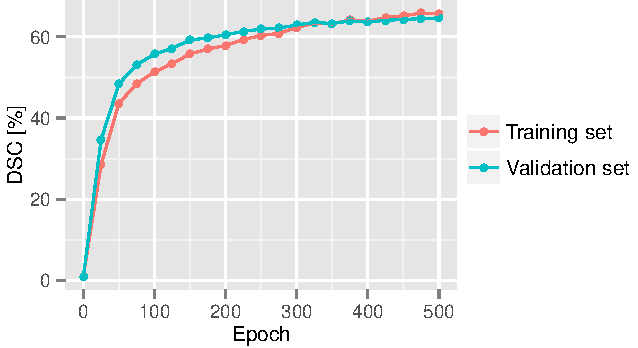
\includegraphics[width=\columnwidth]{figures/ems_progress2}
\caption{Development of mean DSC on the training and test set during training.
Only small improvements can be observed after 500 epochs.}
\end{figure}

We found that our method is not sensitive to the sensitivity ratio $r$. To
confirm, we have calculated ROC curves on the validation set for different
choices of $r$. Also plotted with the threshold marked in the plot, confirming
that the parameter $r$ mostly affects the choice of the threshold used to
binarize the segmentation, but does not affect the performance of the model for
choices between 0.01 and 0.1. Consequently, we have used the same $r$ for all
experiments.

\begin{figure}
\centering
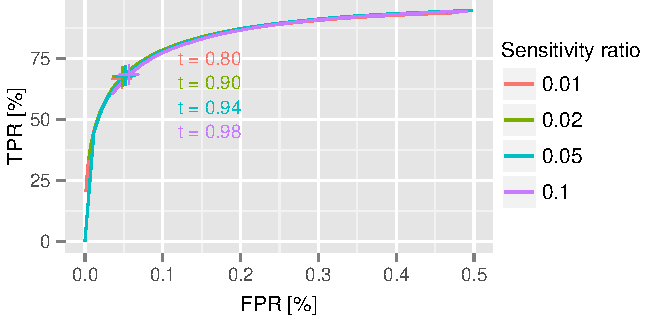
\includegraphics[width=\columnwidth]{figures/roc}
\caption{ROC curves for different sensitivity ratios $r$. A plus marks the TPR
and FPR of the optimal threshold. The ROC curves for different sensitivity
ratios are almost identical and only causes a change of the optimal threshold
$t$, which shows the robustness of our method with respect to the sensitivity
ratio.}
\end{figure}

\subsection{Comparison on Public Data Sets}

In our previous paper \cite{brosch2015}, we showed that approximately 100 images
are required to train the 3-layer CEN without overfitting and we expect the
required number of images to be even higher when adding more layers. Due to the
relatively small size of the training data sets provided by the MICCAI and ISBI
challenges, we trained a CEN with only 3 layers on these data sets, to reduce
the risk of overfitting.

I will have a comparison on the ISBI challenge training set using
leave-one-subject-out cross-validation. To reduce the risk of overfitting, only
trained 3-layer CEN. Describe the data: 5 subjects with 4 time points each.
Winning method did not describe the evaluation process well enough to allow for
an accurate production of the experiments. Therefore, only compare against the
second and third best method. Following they protocol, we performed
leave-one-subject out cross-validation and trained separate models on the GT
masks produced by rater 1 and 2 and compared the model against the masks from
rater 1 and 2, which yields 4 experiments in total: a) trained on rater 1 and
compared against rater 1, b) trained on rater 1 and compared against rater 2, c)
trained on rater 2 and compared against rater 1, and d) trained on rater 2 and
compared against rater 2. Or, for simplicity, only trained on the masks of rater
1 and compared against rater 1 and rater 2 masks. Only 4 subjects per training
fold. To reduce the risk of overfitting, only trained the 3-layer CEN. Table~??
shows a comparison with the other methods.

\begin{table}
\caption{Comparison of our method with the second and third ranked methods from
the ISBI MS lesion segmentation challenge.}
\begin{center}
% \begin{tabular}{llll}
% \toprule
% Method & LTPR & LFPR & DSC \\
% \midrule
% \multicolumn{4}{c}{\textit{Comparison against rater 1}} \\
% \midrule
% Rater 2 & 83.2 & 34.8 & 73.4 \\
% Second &  61.1 & 13.5 & 70.4 \\
% Third \\
% 3-layer CEN \\
% \midrule
% \multicolumn{4}{c}{\textit{Comparison against rater 2}} \\
% \midrule
% Rater 1 & 65.2 & 16.8 & 73.4 \\
% Outlier & 50.1 & 12.7 & 68.1 \\
% Random forest \\
% 3-layer CEN \\
% \bottomrule
% \end{tabular}
% 
% \vspace{1em}
\begin{tabular}{@{}lcccccc@{}}
\toprule
Method &
\multicolumn{3}{c}{Rater 1} &
\multicolumn{3}{c}{Rater 2} \\
& DSC & LTPR & LFPR & DSC & LTPR & LFPR \\
\midrule
Rater 1 & --- & --- & --- & 73.2 & 64.5 & 17.4 \\
Rater 2 & 73.2 & 82.6 & 35.5 & --- & --- & --- \\
Jesson et al. &  70.4 & 61.1 & 13.5 & 68.1 & 50.1 & 12.7 \\
Maier et al. (GT1) & 70 & 53 & 48 & 65 & 37 & 44 \\
Maier et al. (GT2) & 70 & 55 & 48 & 65 & 38 & 43 \\
Our method (GT1) & 68.4 & 74.5 & 54.5 & 64.4 & 63.0 & 52.8 \\
Our method (GT2) & 68.3 & 78.3 & 64.5 & 65.8 & 69.3 & 61.9 \\
\bottomrule
\end{tabular}
\end{center}
Note: The evaluation was performed on the training set using
leave-one-subject-out cross-validation. GT1 and GT2 denote that the model was
trained with the segmentations provided by the first and second rater as the
ground truth, respectively.
% Note: LTPR and LFPR values of the third method are shown in parenthesis to
% indicate that a different method was used to calculate those values, which only
% allows for an approximate comparison with the other methods.
\end{table}

We have also evaluated our method on the MICCAI 2008 lesion segmentation
challenge. Data set consists of T1w, T2w, and FLAIR MRIs of 20 subjects. Due to
the relatively small size of the training data set, we have trained a 3-layer
CEN similar to the ISBI challenge and applied the model to the test data set 1.
The evaluation was performed remotely by the challenge organizers. We placed 5th
in the challenge. The results of the top 8 methods are summarized in
Table~\ref{tab:miccai}. Ranked 6th out of 52 entries.

\begin{table}
\sisetup{
  round-mode = places,
  round-precision = 2}%
\caption{Selected methods out of the 52 entries submitted for evaluation to the
MICCAI 2008 MS lesion segmentation challenge.}
\label{tab:miccai}
\begin{center}
\begin{tabular}{@{}clS[table-format=2.2]S[table-format=2.2]S[table-format=2.2]S[table-format=2.2]@{}}
\toprule
Rank & Method & {Score} & {LTPR} & {LFPR} & {VD} \\
\midrule
1  & Jesson et al. & 86.9386 & 48.70 & 28.25 & 80.15 \\
2  & Guizard et al. \cite{guizard2015}   & 86.1071 & 49.85 & 42.75 & 48.80 \\
4  & Tomas-Fernandez et. al \cite{tomas2015} & 84.464 & 46.9 & 44.6 & 45.60 \\
%5  & Jerman et al.          & 84.1555 \\
6  & Our method    & 84.0743 & 51.55 & 51.25 & 57.75 \\
%8  & Strumia et al.         & 83.9262 \\
%10 & Zhan et al.            & 82.6455 \\
11 & Roura et al.   \cite{roura2015} & 82.3442 & 50.15 & 41.85 & 111.60 \\
13 & Geremia et al. \cite{geremia2010}     & 82.0691 & 55.1 & 74.1 & 48.90 \\
24 & Shiee et al. \cite{shiee2010topology} & 79.8975 & 52.4 & 72.7 & 74.45 \\
%33 & Sudre et al. \cite{Sudre2015} & 77.9601 & 22.3 & 18.1 & 285.6 \\
\bottomrule
\end{tabular}
\end{center}
Note: Only the best entry per method is shown for multiple submission. Columns
LTPR, LFPR, and VD show the mean scores of the two raters in percent. Last
updated: Dec 2, 2015.
\end{table}

\subsection{Comparison of Network Architectures, Modalities Used, and
Competing Methods}

\todo[inline]{Mention also different modalities used and update to reflect new
measures and competing methods.}

To determine the effect of network architecture, we compared the segmentation
performance of three different networks.
Specifically, we trained a 3-layer CEN and two 7-layer CENs, one with shortcut
connections and one without, on the 300 training pairs. The parameters of the
networks are given in Table~\ref{tab:arch3} and Table~\ref{tab:arch7}.
Lesion-TOADS was also included in the comparison as a known standard.
A comparison of the segmentation accuracy of the trained networks and
Lesion-TOADS is summarized in Table~\ref{tab:results1}. All CEN architectures
performed significantly better than Lesion-TOADS in overall segmentation
accuracy, where the improvements of the mean DSC scores ranged from 9\,pts for
the 3-layer CEN to 14\,pts for the 7-layer CEN with shortcut. The
improved segmentation performance was mostly due to a reduction of the false
positives. Lesion-TOADS achieved a mean PPV of only \SI{39.86}{\percent},
whereas the CEN with shortcut achieved a mean PPV of \SI{66.58}{\percent}---an
improvement of 27\,pts. The mean TPRs were roughly the same (slightly less than
\SI{50}{\percent}) for all methods except for the 7-layer CEN with shortcut,
which performed slightly better than the other methods with a mean TPR of
\SI{52.75}{\percent}.

This experiment showed that increasing the depth of the CEN
and adding the shortcut connections improves the segmentation accuracy.
Increasing the depth of the CEN from three layers to seven layers improved the
mean DSC by 2\,pts. The improvement was confirmed to be statistically
significant using a one-sided paired $t$-test ($p\text{-value}=\num{0.002}$).
Adding a shortcut to the network further improved the segmentation
accuracy as measured by the DSC by 3\,pts. A second one-sided paired $t$-test
was performed to confirm the statistical significance of the improvement with a
$p\text{-value} < \num{1e-10}$.

% \begin{itemize}
% \item We used 3 different architectures: 3-layer, 7-layer without shortcuts and
% 7-layer with shortcuts.
% \item 7-layer CEN parameters are summarized in Table~\ref{tab:arch7}.
% \item Comparison of segmentation performance on the test set with 3 different
% architectures and lesionTOADS is shown in Table~\ref{tab:results1}
% \item Even the 3-layer model performs much better than lesionTOADS on average.
% \item Better was confirmed using a one-sided paired t-test. Give the p-value.
% \item Better than lesionTOADS ($p$-value = \num{4.732e-9})
% \item Better than 3-layer ($p$-value = \num{0.002})
% \item Better with shortcut connections ($p$-value = \num{1.566e-11})
% \item Adding more layers also improves performance. T-test.
% \item Adding shortcut connections improves performance. t-test.
% \end{itemize}

\begin{table}[tb]
\caption{Parameters of the 3-layer CEN for the evaluation on the challenge data
sets.}
\label{tab:arch3}
\centering
\begin{tabular}{@{}lccr@{}}
\toprule
Layer type & Kernel Size & \#Filters & \multicolumn{1}{c}{Image Size} \\
\midrule
Input & --- & --- & \num{164x206x156x2}\phantom{0} \\
Convolutional & \num{9x9x9x2} & 32 & \num{156x198x148x32} \\
Deconvolutional & \num{9x9x9x32} & 1 & \num{164x206x156x1}\phantom{0} \\
\bottomrule
\end{tabular}
\end{table}

\begin{table}[tb]
\caption{Parameters of the 3-layer CEN used to evaluate different training
methods.}
\label{tab:arch3}
\centering
\begin{tabular}{@{}lccr@{}}
\toprule
Layer type & Kernel Size & \#Filters & \multicolumn{1}{c}{Image Size} \\
\midrule
Input & --- & --- & \num{164x206x52x2}\phantom{0} \\
Convolutional & \num{9x9x5x2} & 32 & \num{156x198x48x32} \\
Deconvolutional & \num{9x9x5x32} & 1 & \num{164x206x52x1}\phantom{0} \\
\bottomrule
\end{tabular}
\end{table}

\begin{table}[tb]
\caption{Parameters of the 7-layer CEN-s used to evaluate different training
methods.}
\label{tab:arch7}
\centering
\begin{tabular}{@{}lccr@{}}
\toprule
Layer type & Kernel Size & \#Filters & \multicolumn{1}{c}{Image Size} \\
\midrule
Input & --- & --- & \num{164x206x52x2}\phantom{0} \\
Convolutional & \num{9x9x5x2} & 32 & \num{156x198x48x32} \\
Average Pooling & \num{2x2x2} & --- & \num{78x99x24x32} \\
Convolutional & \num{9x10x5x32} & 32 & \num{70x90x20x32} \\
Deconvolutional & \num{9x10x5x32} & 32 & \num{78x99x24x32} \\
Unpooling & \num{2x2x2} & --- & \num{156x198x48x32} \\
Deconvolutional & \num{9x9x5x32} & 1 & \num{164x206x52x1}\phantom{0} \\
\bottomrule
\end{tabular}
\end{table}

\begin{table}
\begin{center}
\caption{Comparison of the segmentation accuracy of different CEN models with
Lesion-TOADS}
\label{tab:results1}
\begin{tabular}{@{}lcccc@{}}
\toprule
Method & DSC [\%] & LTPR [\%] & LFPR [\%] & VD [\%] \\
\midrule
\multicolumn{5}{c}{\textit{Input modalities: T1w and FLAIR}} \\
\midrule
3-layer CEN \cite{brosch2015} & 49.24 & 57.33 & 61.39 & 43.45 \\
7-layer CEN & 52.07 & 43.88 & 29.06 & 37.01 \\ 
7-layer CEN-s & 55.76 & 54.55 & 38.64 & 36.30 \\[0.2em]
Lesion-TOADS \cite{shiee2010topology} & 40.04 & 56.56 & 82.90 & 49.36 \\ 
%SLS \cite{Roura} \\
LST-LGA \cite{schmidt2012automated} & 46.64 & 37.50 & 38.06 & 36.77 \\
LST-LPA \cite{schmidt2012automated} & 46.07 & 48.02 & 52.94 & 41.62 \\
\midrule
\multicolumn{5}{c}{\textit{Input modalities: T1w, T2w, and PDw}} \\
% \midrule
% Method & TPR [\%] & PPV [\%] & DSC [\%] \\
\midrule
7-layer CEN-s & 61.18 & 52.00 & 36.68 & 29.38 \\
EMS \cite{vanleemput2001} & 42.94 & 44.80 & 76.58 & 49.29 \\
\midrule
\multicolumn{5}{c}{\textit{Input modalities: T1w, T2w, FLAIR, and PDw}} \\
% \midrule
% Method & TPR [\%] & PPV [\%] & DSC [\%] \\
\midrule
7-layer CEN-s & 63.83 & 62.49 & 36.10 & 32.89 \\
EMS \cite{vanleemput2001} & 39.70 & 49.08 & 85.01 & 34.51 \\
\bottomrule
\end{tabular}
\end{center}
Note: The table shows the mean of the Dice similarity coefficient (DSC), lesion
true positive rate (LTPR), and lesion false positive rate (LFPR). Because
the volume difference (VD) is not limited to the interval $[0, 100]$, a
single outlier can heavily affect the calculation of the mean. We therefore
excluded outliers before calculating the mean of the VD for all methods.
\end{table}

\subsection{Comparison for Different Lesion Sizes}

% TODO: say it's box plots and outliers are denoted by small black circles.

\todo[inline]{Update groups table to show lesion sizes. Also redo the plots for
lesion sizes. Give a better justification for dividing by lesion size. Small
lesions can be more difficult to miss, while large lesions also come with some
problems.}

To examine the effect of lesion load on segmentation performance, we stratified
the test set into five groups based on their reference lesion loads as
summarized in Table~\ref{tab:groups}. Most segmentation performance measures
deteriorate with lower lesion loads, because when there are only a few true
lesion voxels, even small segmentation errors can translate into large relative
errors. A comparison of segmentation accuracy of a 3-layer CEN and a 7-layer CEN
with shortcut for different lesion loads is illustrated in Fig.~\ref{fig:l1vl2}.
Adding four layers and shortcut connections improved the segmentation accuracy
for all lesion load groups, where the improvements were largest for the highest
lesion loads. In MS, lesion load is strongly correlated with lesion size, which
means that the group with the highest lesion load also contains scans with the
largest lesions. The receptive field of the 3-layer CEN has a size of only
\num{17x17x9} voxels, which reduces its ability to identify very large lesions.
In contrast, the 7-layer CEN has a receptive field size of \num{49x53x26}
voxels, which allows it to learn features that can capture much larger lesions
than the 3-layer CEN. Consequently, the 7-layer CEN is able to learn a feature
set that captures a wider range of lesion sizes, which in turn improves the
segmentation accuracy especially for very high lesion loads, where larger
lesions are also more prevalent.

\begin{table}[tb]
\caption{Lesion load classes as used for the detailed analysis.}
\label{tab:groups}
\centering
\begin{tabular}{@{}lccc@{}}
\toprule
Group & Lesion load [\si{\cubic\milli\metre}] & \#Samples & Lesion size
[\si{\cubic\milli\metre}]\\
\midrule
% 0, 1250, 2500, 3800, 10000
Very low & $[0,3250]$ & 17 \\
Low      & $(3250,6500]$ & 16 \\
Medium & $(6500,10000]$ & 18 \\
High & $(10000,25000]$ & 18 \\
Very high & $> 25000$ & 8 \\
\bottomrule
\end{tabular}
\end{table}

% \begin{itemize}
% \item Analyse where the performance gains come from
% \item 7-layer CEN improves across the board but improvements are particularly
% high for large lesion loads
% \item Large lesion load is also associated with larger lesions
% \item Small filters fail to detect large lesions correctly
% \item 7-layer CEN uses a hierachy of features where each layer represents
% features of a different scale
% \item This allows the detection of a wider spectrum of lesion sizes.
% \item Analyse the relationship of segmentation performance and lesion load
% \item Divided the test set into 5 classes with roughly the same number of
% samples. Classes are (0,1250) ($n=17$), (1250,2500) ($n=16$), (2500, 3800)
% ($n=18$), (3800,10000) ($n=18$), above 10000 ($n=8$). Mention the number of
% samples per class.
% \item CEN outperforms Lesion-TOADS for all lesion load categories, except for
% very high lesion load.
% \item For very high lesion load, no difference to Lesion-TOADS found using
% t-test.
% \item TPR, PPV, DSC for different lesion loads in a table.
% \end{itemize}

% \begin{figure}[tb]
% %\centering
% 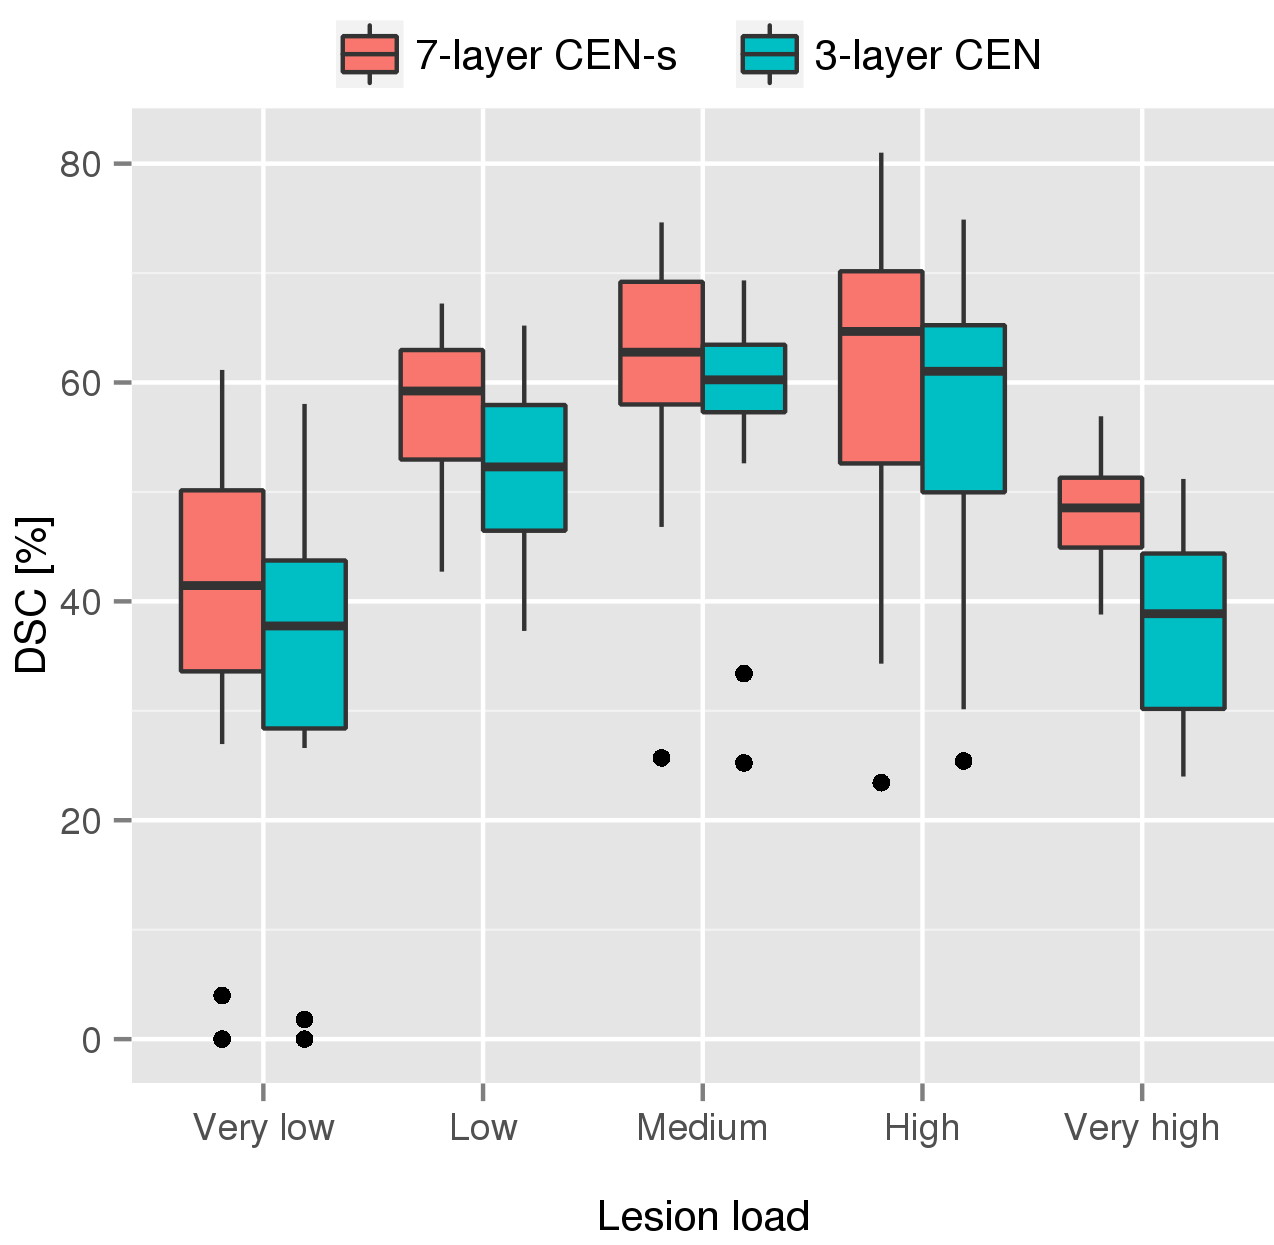
\includegraphics[width=0.92\columnwidth]{figures/boxplot_L1vsL2}
% 
% \caption{Comparison of the segmentation accuracy (DSC) of a 3-layer CEN and a
% 7-layer CEN-s for different lesion load groups. Adding four layers and
% shortcut connections improves the performance across all lesion loads, where the
% improvements are especially large for scans with large lesion loads, which are
% also correlated with lesion size.}
% 
% \label{fig:l1vl2}
% \end{figure}

% \begin{figure*}
% \centering
% 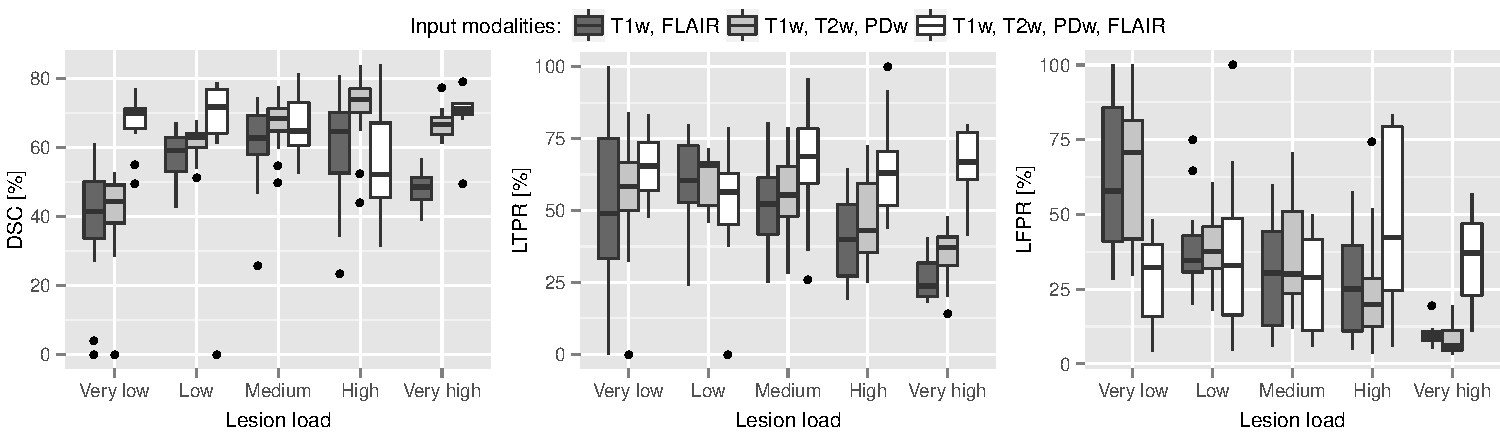
\includegraphics[width=\textwidth]{figures/modalities}
% \caption{Comparison of modalities. No single modality is the most important.
% Combining all four modalities gives significantly better results. Outliers are
% denoted by small black circles.}
% \end{figure*}

% TODO: The small number of scans in the highest load group makes comparing
% across groups difficult. Maybe weaken the statement or point out the
% limitation with sample size.

Fig.~\ref{fig:l2vlt} shows a comparison of the 7-layer CEN with shortcut and
Lesion-TOADS. The CEN approach outperformed Lesion-TOADS for all lesion load
groups, except the group with very high lesion loads, where Lesion-TOADS
achieved a slightly higher mean DSC than the CEN approach, but the difference is
much smaller than the gains in accuracy achieved by the CEN for the other lesion
loads. The 7-layer CEN with shortcut also performed more consistently across
lesion load groups, whereas Lesion-TOADS decreased more strongly in performance
for the smaller lesion loads. As a result, the greatest differences between the
two methods are seen in the lowest lesion load groups.
% However, a two-sided paired $t$-test yielded that
% the difference is not statistically significant ($p\text{-value}=0.2566$).
Table~\ref{tab:result2} shows a more detailed
comparison. While the PPV increased consistently with higher lesion loads for
both methods, the TPR was highest for low to medium lesion loads and decreased
again for high to very high lesion loads. This shows the difficulty for both
methods to correctly identify very large lesions that can extend far into the
white matter.

\begin{figure*}
\centering
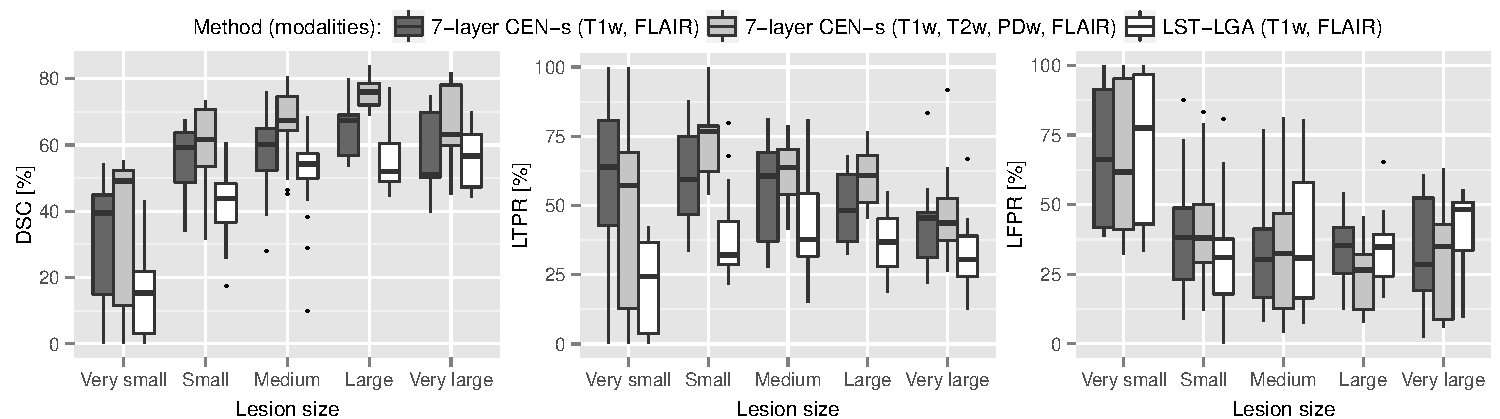
\includegraphics[width=\textwidth]{figures/cen_vs_LGA_size}
\caption{Comparison of our method trained on two different combinations of
modalities and the best performing competing method for different lesion sizes.}
\end{figure*}

% \begin{figure}[tb] 
% %\centering
% 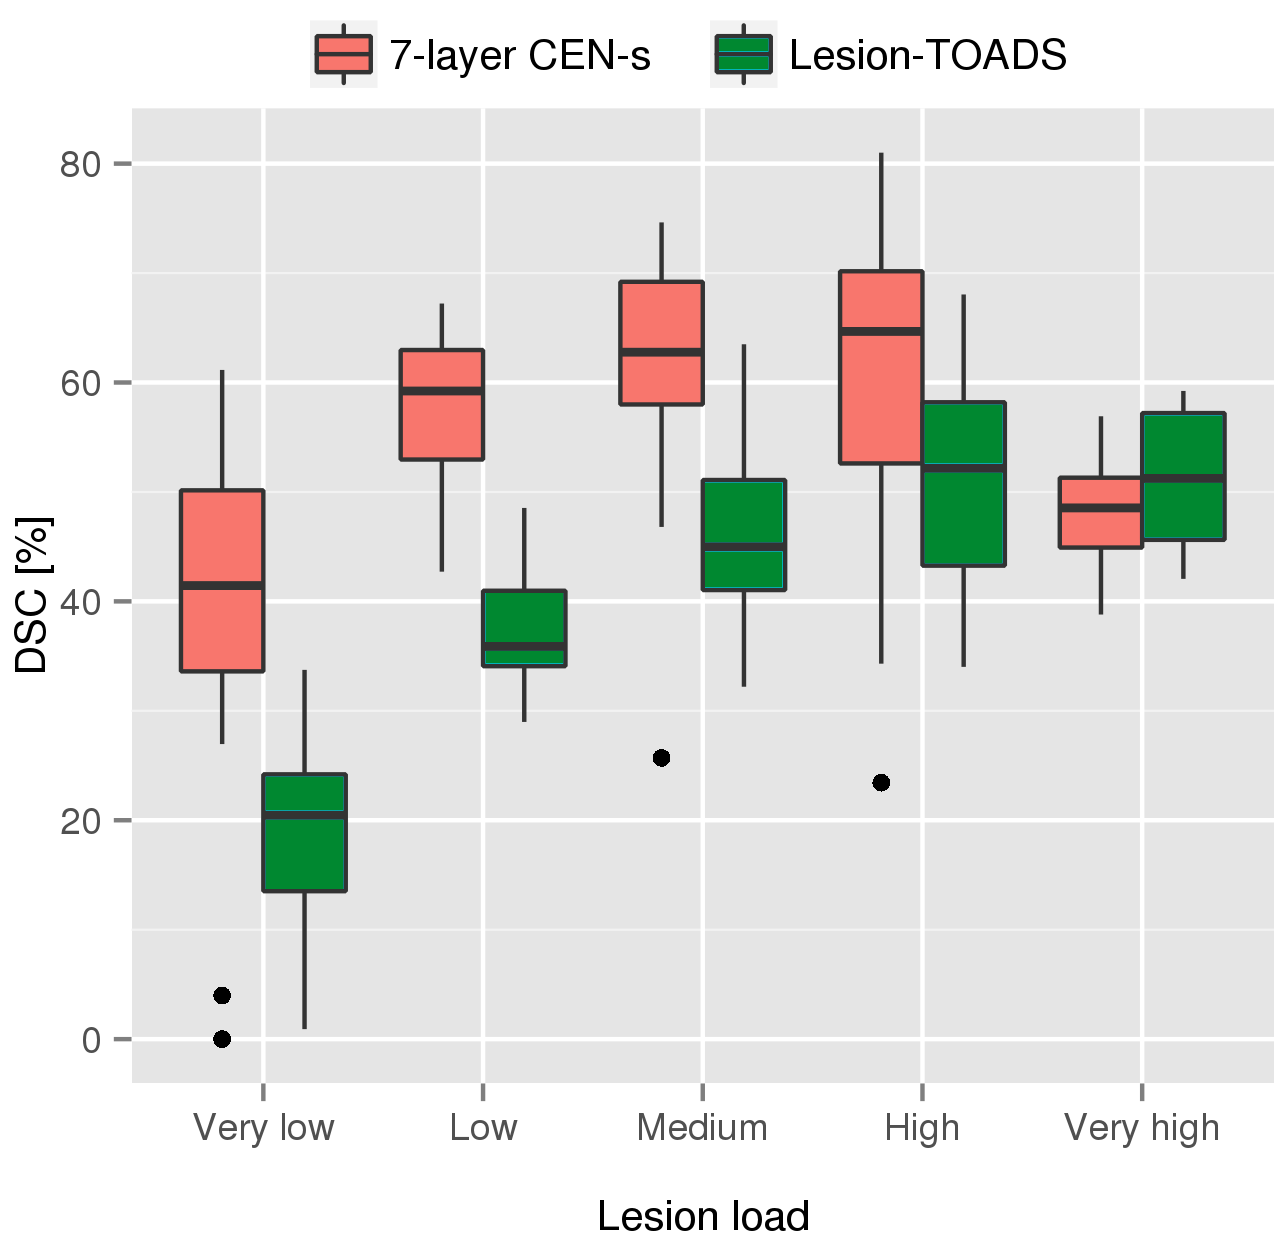
\includegraphics[width=0.92\columnwidth]{figures/boxplot_LTvsL2}
% \caption{Comparison of the segmentation accuracy (DSC) of
% Lesion-TOADS and a 7-layer CEN with shortcut connections for different lesion
% loads. The CEN approach is much more sensitive in detecting small lesions, while
% still being able to detect large lesions.}
% \label{fig:l2vlt}
% \end{figure}

\begin{comment}
\begin{table}
\caption{Comparison of segmentation accuracy for different lesion load
categories.}
\label{tab:result2}
\begin{center}
\begin{tabular}{@{}lcccccc@{}}
\toprule
\multicolumn{1}{@{}l}{Lesion load} & \multicolumn{3}{c}{7-layer CEN-s} &
\multicolumn{3}{c@{}}{Lesion-TOADS}
\\
& TPR & PPV & DSC & TPR & PPV & DSC \\
\midrule
% \phantom{000}$(0,1250]$\phantom{0} & \num{50.00} & \num{41.15} & \num{39.34} &
% \num{49.96} & \num{13.09} & \num{18.86}\\
% $(1250,2500]$\phantom{0} & \num{61.92} & \num{59.01} & \num{57.45} & \num{52.39}
% & \num{29.95} & \num{37.74}\\
% $(2500,3800]$\phantom{0} & \num{57.64} & \num{71.54} & \num{61.31} & \num{54.17}
% & \num{41.83} & \num{46.53}\\
% $(3800,10000]$ & \num{51.14} & \num{81.11} & \num{60.13} & \num{47.97} &
% \num{56.56} & \num{50.76}\\
% $> 10000$ & \num{32.82} & \num{91.95} & \num{48.19} & \num{38.88} & \num{74.6} &
% \num{50.93}\\
Very low & \num{50.00} & \num{41.15} & \num{39.34} &
\num{49.96} & \num{13.09} & \num{18.86}\\
Low & \num{61.92} & \num{59.01} & \num{57.45} & \num{52.39}
& \num{29.95} & \num{37.74}\\
Medium & \num{57.64} & \num{71.54} & \num{61.31} & \num{54.17}
& \num{41.83} & \num{46.53}\\
High & \num{51.14} & \num{81.11} & \num{60.13} & \num{47.97} &
\num{56.56} & \num{50.76}\\
Very high & \num{32.82} & \num{91.95} & \num{48.19} & \num{38.88} & \num{74.6} &
\num{50.93}\\
\bottomrule
\end{tabular}
\end{center}
\end{table}
\end{comment}

% \begin{itemize}
% \item Have some sample images and discuss what we can see here.
% \end{itemize}

\subsection{Qualitative Results}

%TODO: show and discuss filters

\todo[inline]{Update images to show good, mean and bad segmentation. It's more
about showing the range of difficulty in the data set from easy images to
difficult images. If time permits, show some filters and say something about
them.}

A qualitative comparison of segmentation performance for four characteristic
cases is shown in Fig.~\ref{fig:images}. Our method uses a combination of
automatically learned intensity and appearance features, which makes it
inherently robust to noise (see Fig.~\ref{fig:images}a), while still being able
to detect small isolated lesions (see Fig.~\ref{fig:images}b). Furthermore, our
method is able to learn a wide spectrum of lesion shapes and appearances from
training data, which allows our method to correctly identify multiple different
types of MS lesions. For example, our method was able to correctly identify a
large T1 black hole that was partially missed by Lesion-TOADS (see
Fig.~\ref{fig:images}c), which has a known limitation of sometimes
misclassifying T1 black holes due to different intensity profiles of partially
overlapping T1 hypointense and T2 hyperintense regions \cite{shiee2010topology}.
Figure~\ref{fig:images}d shows one of the most challenging cases for our method.
Very large lesions can extend beyond the size of the receptive field of the CEN,
which reduces its ability to extract characteristic lesion features.
Consequently, in some cases our method can underestimate the size of very large
lesions.

\begin{comment}
\begin{figure*}
\begin{tikzpicture}[node distance=1.5cm and 0.1\textwidth,
  font=\footnotesize, on grid]
  
\node[inner sep=0] (image1) {
  \includegraphics[width=\textwidth]{figures/i10_W9401S01_small_lesion_vessel_outlier}
};
\node[above=of image1,xshift=-0.05\textwidth,align=center] (l3) {%
3-layer CEN\\(T1,FL)};
\node[right=of l3,align=center] (l7) {7-layer CEN-s\\(T1,FL)};
\node[right=of l7,align=center] (l7s){7-layer CEN-s\\(T1,FL,T2,PD)};
\node[right=of l7s,align=center] (ems) {\phantom{g}EMS\phantom{g}\\(T1,T2,PD)};
\node[right=of ems,align=center] (lt) {L-TOADS\\(T1,FL)};
\node[right=of lt,align=center] (LST) {\phantom{g}LST-LGA\phantom{g}\\(T1,FL)};
\node[left=of l3] (pd) {PD-weighted};
\node[left=of pd] (t2) {T2-weighted};
\node[left=of t2] (flair) {\phantom{g}FLAIR\phantom{g}};
\node[left=of flair] (t1) {T1-weighted};

\node[inner sep=0, below=2.4cm of image1] (image2) {
  \includegraphics[width=\textwidth]{figures/i10_W9702S07_poor_contrast_lesions}
};

\node[inner sep=0, below=2.4cm of image2] (image3) {
  \includegraphics[width=\textwidth]{figures/i10_W9902S07_high_LL_improvements}
};

\end{tikzpicture}
\caption{Comparison of segmentation results of different segmentation methods
for 3 subjects. The first and the second row highlight the difficulty}
\end{figure*}
\end{comment}

\begin{figure}
\begin{tikzpicture}[node distance=2.1cm and 0.333\columnwidth,
  font=\footnotesize, on grid]
\node[inner sep=0] (image1) {
  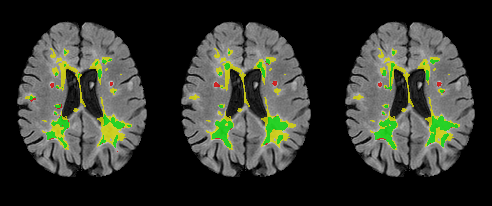
\includegraphics[width=\columnwidth]{figures/p50s35_large_lesions}
};
\node[above=of image1] (l7) {7-layer CEN};
\node[left=of l7] {3-layer CEN};
\node[right=of l7] {7-layer CEN-s};

\begin{scope}[xshift=0.333\columnwidth]
\draw[white,thick] (-12pt,-15pt) circle (9pt);
\draw[white,thick] (15pt,-15pt) circle (10pt);
\end{scope}
\begin{scope}[xshift=-0.333\columnwidth]
\draw[white,thick] (-12pt,-15pt) circle (9pt);
\draw[white,thick] (15pt,-15pt) circle (10pt);
\end{scope}
\draw[white,thick] (-12pt,-15pt) circle (9pt);
\draw[white,thick] (15pt,-15pt) circle (10pt);
\end{tikzpicture}
\caption{Large lesion problematic for 3-layer CEN due to limited size of the
receptive field. The adding layers increases the size of the receptive field,
which improves the detection of very large lesions.}
\label{fig:large}
\end{figure}

\begin{figure}
\begin{tikzpicture}[node distance=2.1cm and 0.333\columnwidth,
  font=\footnotesize, on grid]
\node[inner sep=0] (image1) {
  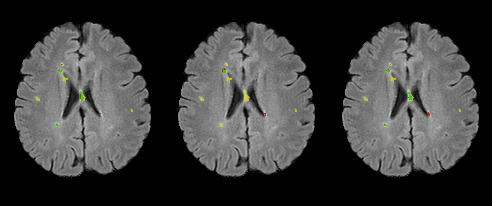
\includegraphics[width=\columnwidth]{figures/p25s35_small_lesions}
};
\node[above=of image1] (l7) {7-layer CEN};
\node[left=of l7] {3-layer CEN};
\node[right=of l7] {7-layer CEN-s};
\begin{scope}[xshift=0.3333\columnwidth]
\draw[white,thick] (-12.5pt,-11pt) circle (4pt);
\draw[white,thick] (0pt,4pt) circle (6pt);
\draw[white,thick] (-10pt,20pt) circle (3pt);
\end{scope}
\begin{scope}[xshift=-0.3333\columnwidth]
\draw[white,thick] (-12.5pt,-11pt) circle (4pt);
\draw[white,thick] (0pt,4pt) circle (6pt);
\draw[white,thick] (-10pt,20pt) circle (3pt);
\end{scope}
\draw[white,thick] (-12.5pt,-11pt) circle (4pt);
\draw[white,thick] (0pt,4pt) circle (6pt);
\draw[white,thick] (-10pt,20pt) circle (3pt);
\end{tikzpicture}

\caption{Comparison of segmentation performance of different CEN architectures
for small lesions. The white circles indicate lesions that were detected by the
3-layer CEN and the 7-layer CEN with shortcut. Increasing the size of the
receptive field decreases the sensitivity to small lesions. The addition of a
shortcut allows the detection of small lesions, while still being able
to detect large lesions (see Fig.~\ref{fig:large}).}
\label{fig:small}
\end{figure}

\begin{comment}
\begin{figure*}
%\centering
\hspace*{-5pt}
\subfloat[Robustness to noise] {
\begin{tikzpicture}[node distance=1.5cm and 0.2\columnwidth,
  font=\footnotesize, on grid]
  
\node[inner sep=0] (image) {
  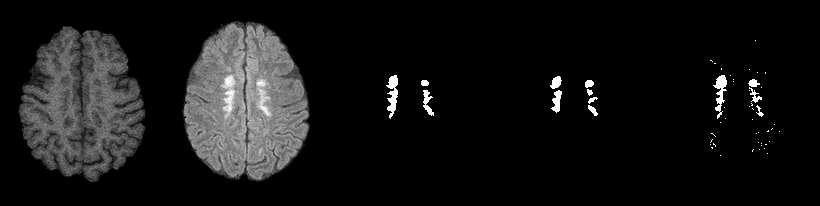
\includegraphics[width=\columnwidth]{figures/p15s34_robust_to_noise3}
  };
\node[above=of image] (gt) {\phantom{g}Ground truth\phantom{g}};
\node[left=of gt] (flair) {\phantom{g}FLAIR\phantom{g}};
\node[left=of flair] {T1-weighted};
\node[right=of gt,align=center] (cen) {\phantom{g}Our method\phantom{g}};
\node[right=of cen,align=center] {Lesion-\\ TOADS};

\end{tikzpicture}
}
\subfloat[Sensitivity to small isolated lesions.] {
\begin{tikzpicture}[node distance=1.5cm and 0.2\columnwidth,
  font=\footnotesize, on grid]
  
\node[inner sep=0] (image) {
  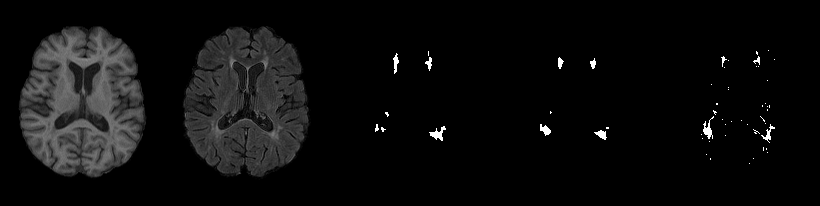
\includegraphics[width=\columnwidth]{figures/p17s29_noisy_lesionTOADS}};
  \node[above=of image] (gt) {\phantom{g}Ground truth\phantom{g}};
\node[left=of gt] (flair) {\phantom{g}FLAIR\phantom{g}};
\node[left=of flair] {T1-weighted};
\node[right=of gt,align=center] (cen) {\phantom{g}Our method\phantom{g}};
\node[right=of cen,align=center] {Lesion-\\ TOADS};

\draw[green, thick] (-7pt,-3.5pt) circle (3pt);
\begin{scope}[xshift=0.2\columnwidth]
\draw[green, thick] (-7pt,-3.5pt) circle (3pt);
\end{scope}

\end{tikzpicture}
}\\
\hspace*{-5pt}
\subfloat[Example of a T1 black hole that was correctly identified by our
method] {
\begin{tikzpicture}
\node[inner sep=0pt] {
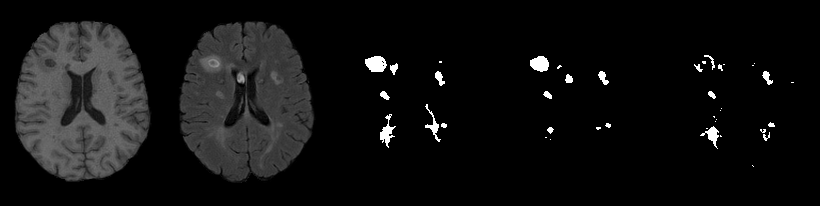
\includegraphics[width=\columnwidth]{figures/p36s30_blackhole}};
\draw[red,thick] (-10pt,12pt) circle (7pt);
\begin{scope}[xshift=-0.2\columnwidth]
\draw[red,thick] (-10pt,12pt) circle (7pt);
\end{scope}
\begin{scope}[xshift=-0.4\columnwidth]
\draw[red,thick] (-10pt,12pt) circle (7pt);
\end{scope}
\begin{scope}[xshift=0.2\columnwidth]
\draw[red,thick] (-10pt,12pt) circle (7pt);
\end{scope}
\begin{scope}[xshift=0.4\columnwidth]
\draw[red,thick] (-10pt,12pt) circle (7pt);
\end{scope}
\end{tikzpicture}
}
\subfloat[Very large lesions can be underestimated] {
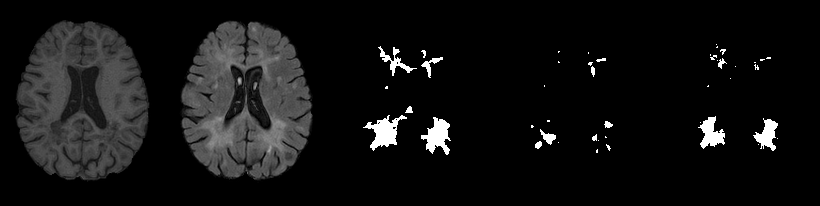
\includegraphics[width=\columnwidth]{figures/p54s32_large_lesions}
}

\caption{Four cases illustrating the strengths and limitations of our method
compared to Lesion-TOADS. Our method is inherently robust to noise (a), while
still being able to detect small isolated lesions (b). Furthermore, our method
is able to detect multiple different types of lesions correctly (e.g.,
T1 black holes). However, in some cases our method can underestimate the size
of very large lesions (d).}

\label{fig:images}
\end{figure*}
\end{comment}

\begin{comment}
\subsection{BioMS Data Set}

\begin{table}
\caption{Training results on the BioMS data set using 150 and 250 images for
training.}
\begin{center}
\begin{tabular}{llcc}
\toprule
Pre-training & Fine-tuning & Training DSC & Test DSC \\
\midrule
With dropout & Hessian-free (150) & 67.1 & 61.7 \\
With dropout & Hessian-free (250) & 68.0 & 62.8 \\
Without dropout & Hessian-free (150) & 66.5 & 61.7 \\
With dropout & AdaDelta (150) & 65.9 & 60.6 \\
Without dropout & AdaDelta (150) & 66.0 & 60.6 \\
\bottomrule
\end{tabular}
\end{center}
Notes: No comparison with
state-of-the-art methods are available here. The effect of dropout in the
pre-training phase on the final result is negligible. Hessian-free is slightly
better than AdaDelta and does not require the tuning of parameters. However,
Hessian-free optimization does not support dropout, which might be important
for regularization when the data set size is small or the number of layers and
filters is high.
\end{table}
\end{comment}

% \subsection{On a small data set}
% 
% Include MICCAI challenge results, because it was a comparison with more methods.

\begin{comment}
\subsection{Evaluation of Training Methods}

We have evaluated the impact of different training and initialization methods on
the performance of the trained network using the example of a 7-layer CEN. The
network architecture is summarized in Table~\ref{tab:arch7}. All methods have
hyperparameters, which can be difficult to choose. To find a good set of
hyperparameters for each algorithm (except for Hessian-free), we first trained
the model for 20 epochs with the hyperparameters shown in
Table~\ref{tab:parameters}. We then used the set of parameters that produced the
lowest error on the training set to further fine-tune the model for 500 epochs.
This tuning procedure favors algorithms that are robust to the choice of the
hyperparameters or can make substantial progress within the first few epochs,
which are both desirable properties of a training method for which
time-consuming parameter tuning using a large number of epochs and
cross-validation is not feasible. As is the case for the training on large data
sets on high-resolution 3D medical images. The hyperparameters of the
Hessian-free optimization are very robust to the choice of input data. We found
that tuning these parameters is not necessary. Another difference of the
Hessian-free optimization compared to the other methods is that HF is able to
make more progress within an epoch, albeit at the cost of more time-consuming
updates. To compensate, we trained HF for only 22 epochs. Parameter estimation
and fine-tuning of the model required 2.9 GB of GPU memory and took
approximately 42 hours on a single NVIDIA GeForce GTX 780 graphics card.
However, once the model has been trained, segmentation of an entire 3D image can
be performed in less than half a seconds.

\begin{table}
\caption{Algorithm parameters}%
\label{tab:parameters}
\begin{center}
\begin{tabular}{@{}lp{0.7\columnwidth}@{}}
\toprule
Algorithm & Parameters \\
\midrule
SGD \cite{LeCun1998} & $\text{learning rate} \in \{\num{e-3}, \num{e-4}, \num{e-5},
\num{e-6}\},\newline \text{momentum} = 0.9$ \\

AdaGrad \cite{duchi2011adaptive} & $\alpha \in \{\num{e-4}, \num{e-5},
\num{e-6}, \num{e-7}\}, \epsilon = \num{e-11}$ \\

Adam \cite{kingma2014adam} & $\alpha \in \{\num{3e-5}, \num{e-5}, \num{e-6},
\num{e-7}\}$, $\beta_1 = 0.1$, \newline $\beta_2 = 0.001$, $\epsilon = \num{e-11}$ \\

AdaDelta \cite{zeiler2012adadelta} & $\epsilon \in \{\num{e-9}, \num{e-10},
\num{e-11}\}, \rho= 0.95$
\\

RMSProp \cite{dauphin2015rmsprop} & $\epsilon \in \{\num{e-4}, \num{e-5},
\num{e-6}, \num{e-7}\}, \alpha = 0.9 $\\

Hessian-free \cite{martens2010deep} & $\lambda_0 = 1, \zeta = 0.9$ \\
\bottomrule
\end{tabular}
\end{center}
Note: Please refer to the respective paper for a detailed description of the
hyperparameters.
\end{table}

Figure~\ref{fig:methods} shows a comparison of Dice similarity coefficients
calculated on the test set after training the 7-layer CEN with different
optimization methods as well as with and without pre-training. The results for
SGD are not included in the figure, because we were not able to find a learning
rate for which SGD can make notable progress.
\begin{itemize}
\item SGD is not included because the training method failed to make notable
progress
\item A possible explanation is that the parameters of different layers vary
greatly in magnitude and therefore require different learning rates
\item However, SGD used the same learning rate for all layers and the tuning
phase was not able to find a learning rate that works for all layers
\item In addition, none of the first-order methods were able to train the
CEN without pre-training, which further highlights the difficulty of training deep
CNNs on sparse segmentations.
\item We found that pre-training is crucial to alleviate the difficulty of
training deep CNNs with very unbalanced classes.
\item The training algorithms AdaDelta, Adam, Hessian-free and RMSProp perform
roughly the same with only AdaGrad notably worse than the other methods.
\item Hessian-free optimization was the only method that did not require
pre-training, where the results with pre-training are still slightly better than
without pre-training
\end{itemize}  

\begin{figure}[tb]
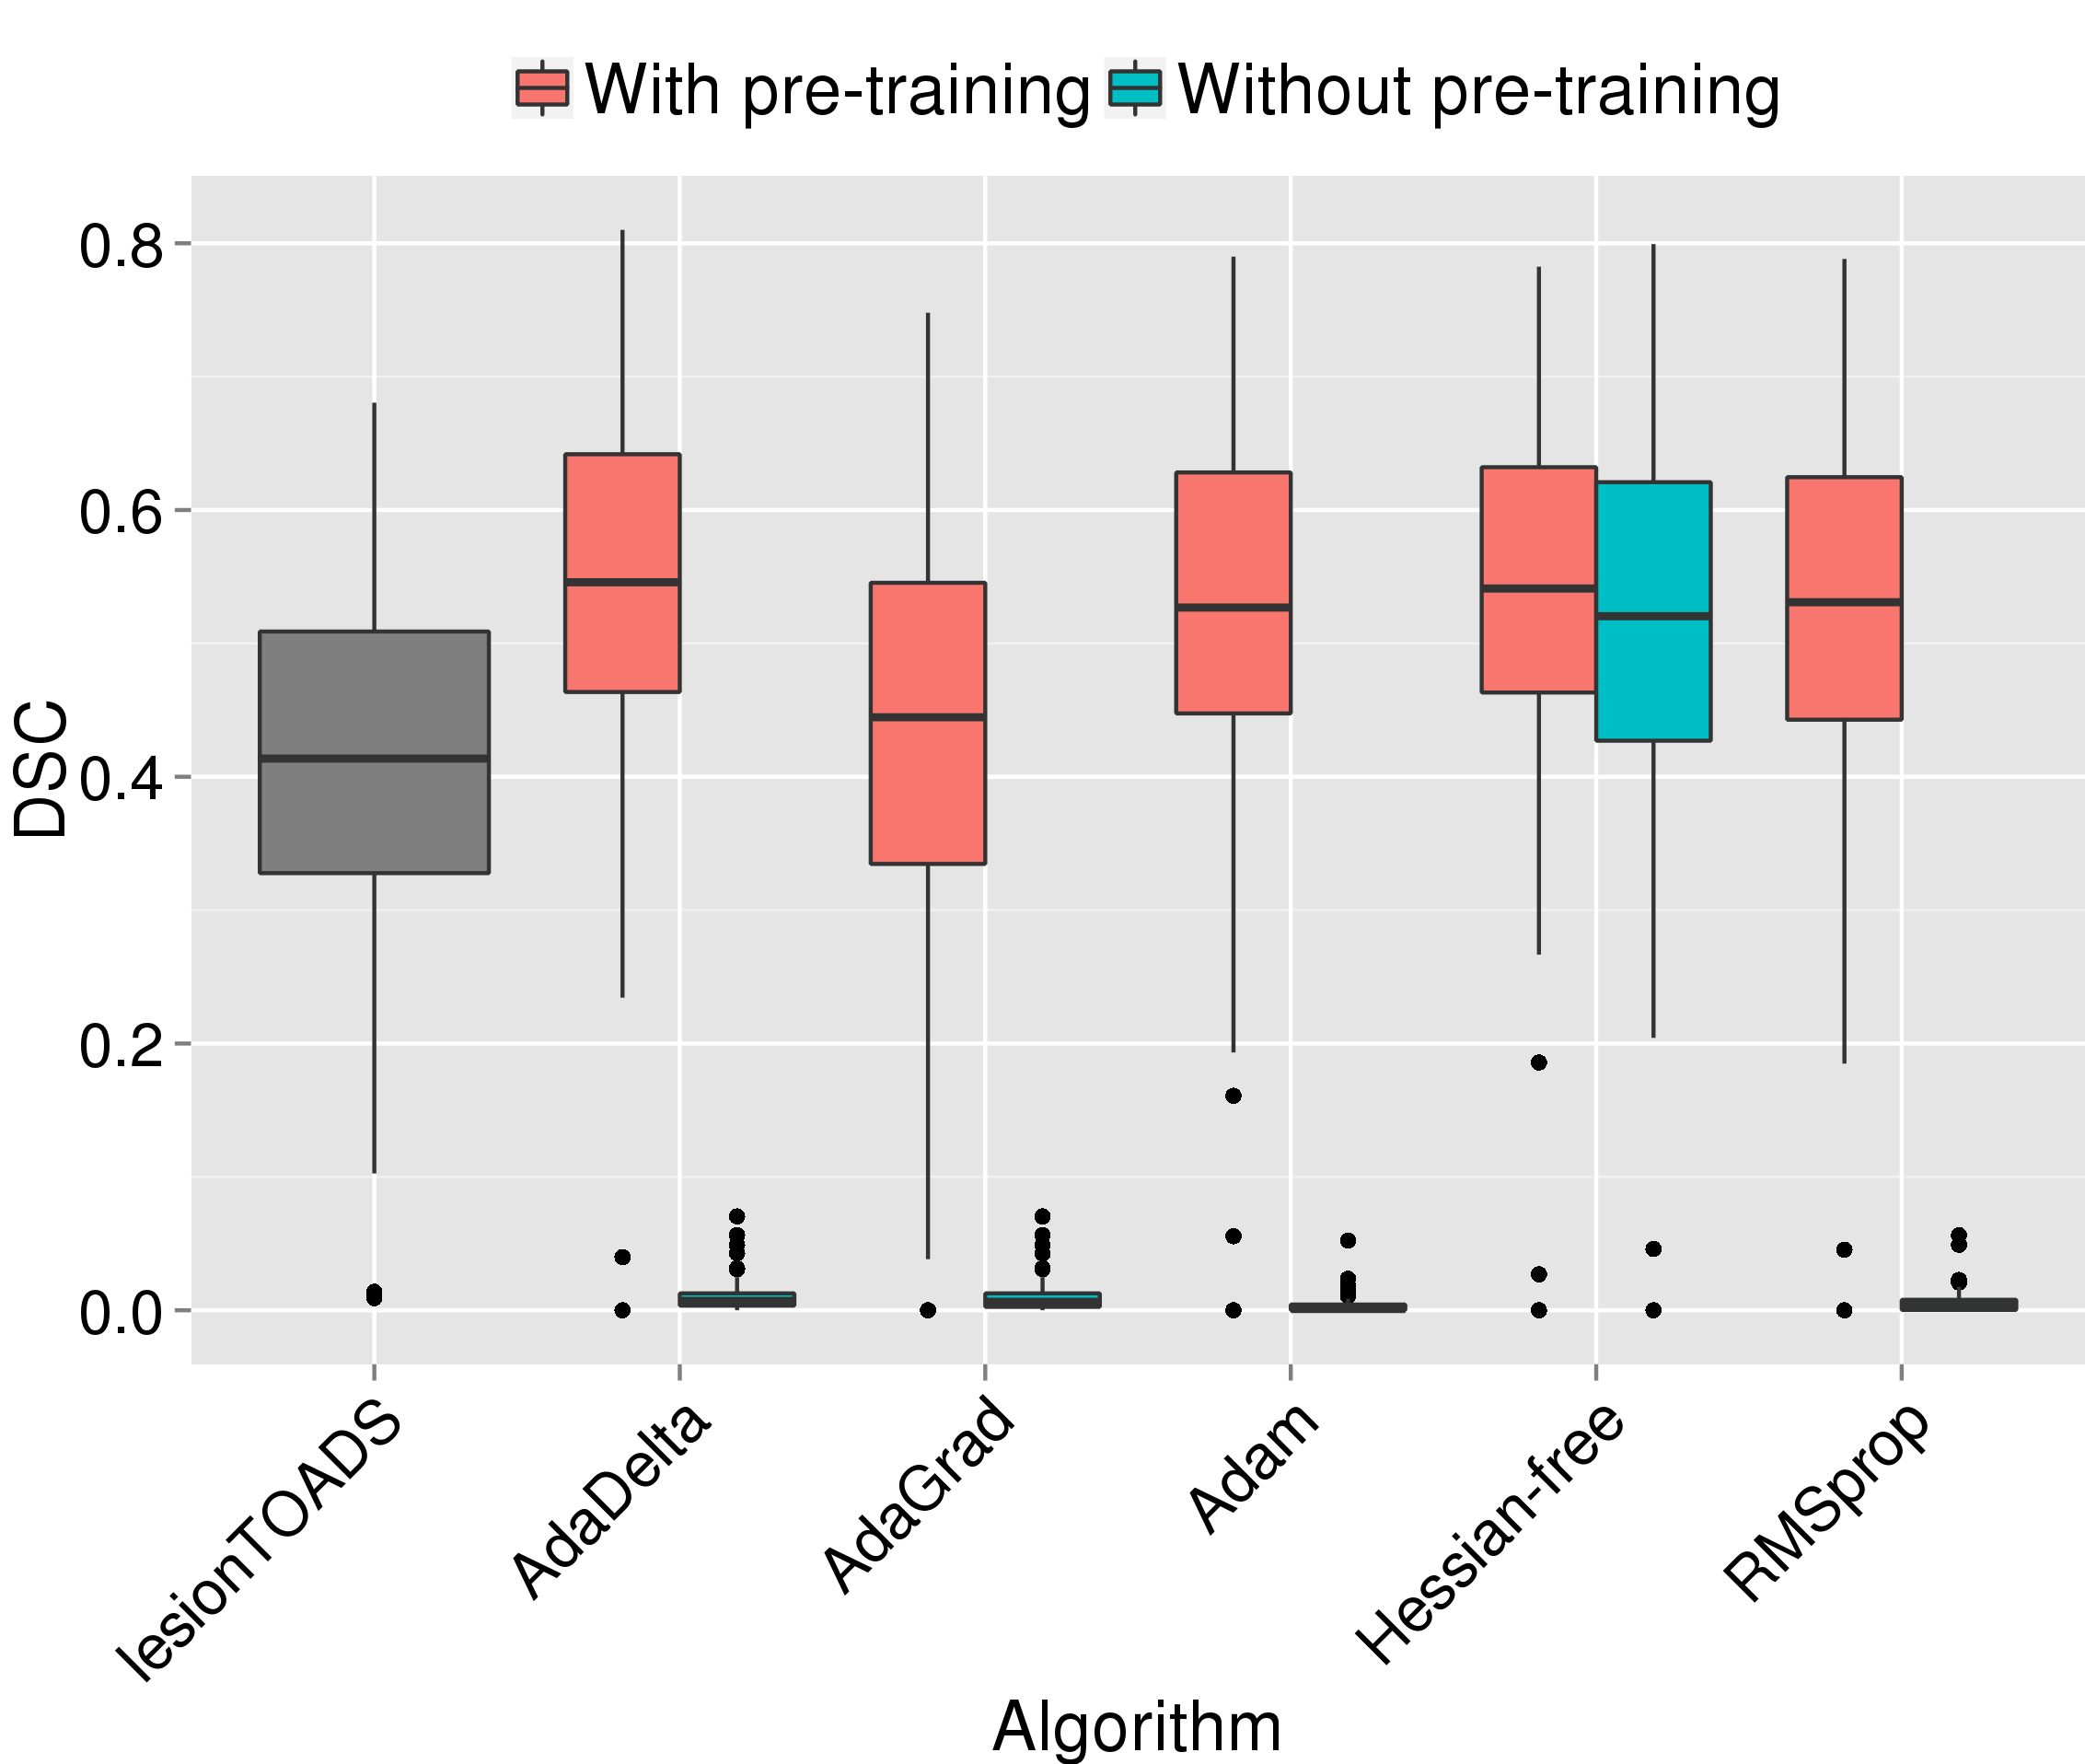
\includegraphics[width=\columnwidth]{figures/methods2}
\caption{Comparison of different training methods with pre-training (left) and
without pre-training (right). Hessian-free is the only method that does not
require pre-training to train the model. With pre-training, AdaDelta, Adam,
Hessian-free, and RMSprop consistently learn models that perform significantly
better than lesionTOADS.}
\label{fig:methods}
\end{figure}

A more detailed comparison of the 7-layer CEN trained with different
optimization algorithms and lesionTOADS is summarized in Table~\ref{tab:results1}.
\begin{itemize}
\item TPR is comparable to lesionTOADS, whereby only the CEN trained with
AdaDelta is able to achieve a higher TPR than lesionTOADS
\item Advantage of CEN model is the much reduces number of false positives,
which results in a significantly higher PPV.
\item All methods, except for AdaGrad, outperform lesionTOADS in terms of the
DCS by more than \SI{10}{\percent}. The best performing method achieves a DSC of
\num{54.02} compared to a DSC of \num{40.04} achieved by lesionTOADS on this
challenging data set.
\end{itemize}

\begin{table}
\sisetup{separate-uncertainty=true,detect-weight=true,detect-inline-weight=math}
\begin{center}
\caption{Comparison of the segmentation accuracy of a 7-layer CEN trained with
different algorithms and lesionTOADS}
\label{tab:results1}
\begin{tabular}{@{}lccc@{}}
\toprule
Algorithm & TPR [\%] & PPV [\%] & DSC [\%] \\
\midrule
AdaDelta & \textbf{\num{52.75+-20.31}} & \num{66.58+-20.71} &
\textbf{\num{54.02+-15.24}} \\
AdaGrad & \num{42.14+-18.88} & \num{54.65+-20.24} & \num{43.21+-15.05} \\
Adam & \num{47.41+-18.96} & \textbf{\num{70.33+-20.98}} & \num{51.93+-15.08} \\
Hessian-free & \num{49.21+-18.76} & \num{68.33+-21.12} & \num{52.65+-15.09} \\
RMSprop & \num{47.9+-20.53} & \num{69.12+-20.78} & \num{51.46+-15.77} \\[0.4em]
lesionTOADS & \num{49.83+-14.79} & \num{39.86+-20.95} & \num{40.04+-14.86} \\
\bottomrule
\end{tabular}
\end{center}
Note: The table shows the mean and standard deviation of the true positive rate
(TPR), positive predictive value (PPV), and Dice similarity coefficient (DSC).
All experiments were performed with pre-training and evaluated on the test set.
\end{table}

\subsection{Evaluation of Network Architectures}

In a second experiment, we evaluated the impact of the network architecture on
the segmentation performance. Therefore, we have trained different networks with
varying number of layers and with and without shortcut connections between the
convolutional and deconvolutional pathway. Table~\ref{tab:arch15} shows the
parameters of a 15-layer CEN. We have used the same parameters for the 11-layer,
7-layer, and 3-layer CENs with the respective layers removed.
\begin{itemize}
\item Shortcut connections are increasingly more important with increasing
depth of the network
\item The DSC decreases with depth without shortcut while it increases with
shortcuts
\item After 11 layers, the network performance does not increase on the test set
as the network starts to overfit more
\item Either more training data or better regularization methods are needed to
train very deep models
\end{itemize}

\begin{table}[tb]
\caption{Parameters of the 15 layers of the CENs used to evaluate different
network architectures.}
\label{tab:arch15}
\begin{center}
\begin{tabular}{@{}lccr@{}}
\toprule
Layer type & Kernel size & Filters & \multicolumn{1}{c}{Image size} \\
\midrule
Input & --- & --- & \num{164x206x52x2}\phantom{0} \\
Convolutional & \num{9x9x5x2} & 32 & \num{156x198x48x32} \\
Average Pooling & \num{2x2x2} & --- & \num{78x99x24x32} \\
Convolutional & \num{9x10x5x32} & 32 & \num{70x90x20x32} \\
Average Pooling & \num{2x2x1} & --- & \num{35x45x20x32} \\
Convolutional & \num{8x10x5x32}  & 32 & \num{28x36x16x32} \\
Average Pooling & \num{2x2x1} & --- & \num{14x18x16x32} \\
Convolutional & \num{7x11x9x32}  & 32 & \num{8x8x8x32} \\
Deconvolutional & \num{7x11x9x32}  & 32 & \num{14x18x16x32} \\
Unpooling & \num{2x2x1}       & --- & \num{28x36x16x32} \\
Deconvolutional & \num{8x10x5x32} & 32 & \num{35x45x20x32} \\
Unpooling & \num{2x2x1}       & --- & \num{70x90x20x32} \\  
Deconvolutional & \num{9x10x5x32} & 32 & \num{78x99x24x32} \\
Unpooling & \num{2x2x2} & --- & \num{156x198x48x32} \\
Deconvolutional & \num{9x9x5x32} & 1 & \num{164x206x52x1}\phantom{0} \\
\bottomrule
\end{tabular}
\end{center}
Note: Networks with fewer layer use the same parameters as the 15-layer
CEN, where the missing layers are simply removed.
\end{table}

Analysis of different training set sizes
\begin{itemize}
\item Varying number of training samples
\item With dropout and without (regularization)
\item Performed on most promising architecture
\item Possible outcome: to harsh regularization decreases performance when
enough training data is available but improves performance for small data sets
due to the reduction of overfitting
\end{itemize}
\end{comment}

% \begin{table}
% \caption{Preliminary segmentation results on the Bravo data set.}
% \begin{center}
% \begin{tabular}{lc}
% \toprule
% Method & Training and test DSCs \\
% \midrule
% Input pre-training, 1-layer CNN &  41.63 / 42.76 \\[0.25em]
% No pre-training, 2-layer CNN & 51.88 / 46.93 \\
% Joint pre-training, 2-layer CNN & 44.52 / 43.82 \\
% Input pre-training, 2-layer CNN & 51.02 / 46.58 \\[0.25em]
% Input pre-training, 4-layer CNN & 59.60 / 46.14 \\[0.25em]
% Lesion-TOADS & \phantom{00.}--- / 34.87 \\
% \bottomrule
% \end{tabular}
% \end{center}
% Note: All tests were performed with Hessian-free optimization. Pre-training was
% always performed with dropout.
% \end{table}

\begin{comment}


To allow for a direct comparison with state-of-the-art lesion segmentation
methods, we evaluated our method on the FLAIR, T1-, and T2-weighted MRIs of the
20 publicly available labeled cases from the MS lesion segmentation challenge
2008 \cite{styner20083d}, which we downsampled from the original isotropic voxel
size of \SI{0.5}{\cubic\milli\metre} to an isotropic voxel size of
\SI{1.0}{\cubic\milli\metre}. In addition, we evaluated our method on an
in-house data set from an MS clinical trial of 500 subjects split equally into
training and test sets. The images were acquired from 45 different scanning
sites. For each subject, the data set contains T2- and PD-weighted MRIs with a
voxel size of \SI{0.937x0.937x3.000}{\milli\metre}. The main preprocessing steps
included rigid intra-subject registration, brain extraction, intensity
normalization, and background cropping.

We used a CEN with 32 filters and filter sizes of \num{9x9x9} and \num{9x9x5}
voxels for the challenge and in-house data sets, respectively. Training on a
single GeForce GTX 780 graphics card took between 6 and 32 hours per model
depending on the training set size. However, once the network is trained,
segmentation of trimodal 3D volumes with a resolution of, e.g.,
\num{159x201x155} voxels can be performed in less than one second. As a
rough\footnote{Ciresan et al. used a more complex network that is composed of 11
layers. However, their network was trained on much smaller images, which roughly
compensates for the increased complexity.} comparison, Ciresan et al.
\cite{Ciresan2012} reported that their patch-based method required 10 to 30
minutes to segment a single 2D image with a resolution of \num{512x512} voxels
using four graphics cards, which demonstrates the large speed-ups gained by
processing entire volumes.

% \begin{figure}[tb]
% \centering
% \small
% \def\MRIwidth{0.15\textwidth}
% 
% \begin{tikzpicture} 
% \tikzstyle{leftlabel}=[rotate=90, align=center,overlay,above]
% 
% \matrix [matrix of nodes, nodes={anchor=center, inner sep=1pt}] {
%         &[4pt] FLAIR & T1w & T2w & Ground truth & Our method \\[4pt]
% \node[leftlabel] {CHB\,07\\(DSC\,=\,\SI{60.58}{\percent})}; &
% 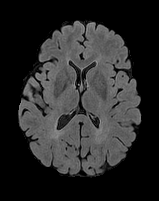
\includegraphics[width=\MRIwidth]{figures/CHB07-FLAIR-s88} &
% 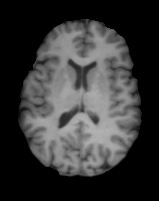
\includegraphics[width=\MRIwidth]{figures/CHB07-T1w-s88} &
% 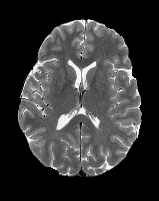
\includegraphics[width=\MRIwidth]{figures/CHB07-T2w-s88} &
% 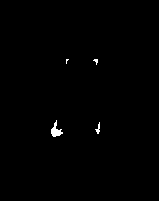
\includegraphics[width=\MRIwidth]{figures/CHB07-gold-s88} &
% 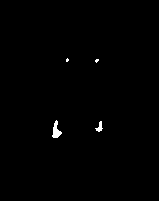
\includegraphics[width=\MRIwidth]{figures/CHB07-pred-s88} \\
% \node[leftlabel] {CHB\,04\\(DSC\,=\,\SI{61.37}{\percent})}; &
% 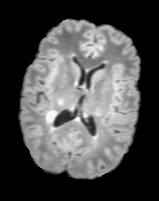
\includegraphics[width=\MRIwidth]{figures/CHB04-FLAIR-s85} &
% 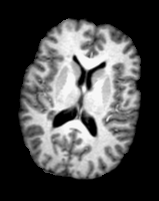
\includegraphics[width=\MRIwidth]{figures/CHB04-T1w-s85} &
% 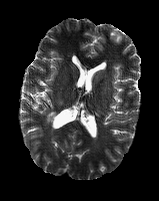
\includegraphics[width=\MRIwidth]{figures/CHB04-T2w-s85} &
% 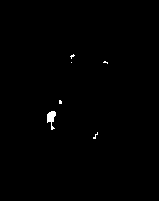
\includegraphics[width=\MRIwidth]{figures/CHB04-gold-s85} &
% 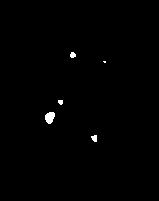
\includegraphics[width=\MRIwidth]{figures/CHB04-pred-s85} \\
% \node[leftlabel] {UNC\,09\\(DSC\,=\,\SI{9.01}{\percent})}; &
% 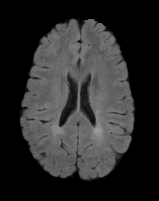
\includegraphics[width=\MRIwidth]{figures/UNC09-FLAIR-s89} &
% 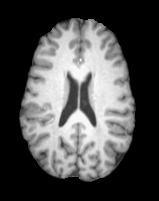
\includegraphics[width=\MRIwidth]{figures/UNC09-T1w-s89} &
% 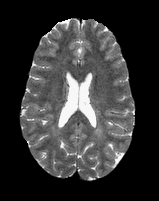
\includegraphics[width=\MRIwidth]{figures/UNC09-T2w-s89} &
% 
\includegraphics[width=\MRIwidth]{figures/UNC09-gold-s89} &
% 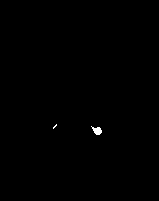
\includegraphics[width=\MRIwidth]{figures/UNC09-pred-s89} \\
% };
% \end{tikzpicture}
% 
% \caption{Example segmentations of our method for three different subjects from
% the challenge data set. Our method performed well and consistently despite the
% large contrast differences seen between the first two rows. In the third row,
% our method also segmented lesions that have similar contrast, but these regions
% had not been identified as lesions by the manual rater, which highlights the
% difficulty in distinguishing focal lesions from diffuse damage, even for
% experts.}
% 
% \label{fig:segmentation}
% \end{figure}

We evaluated our method on the challenge data set using 5-fold
cross-valida\-tion and calculated the true positive rate (TPR), positive
predictive value (PPV), and Dice similarity coefficient (DSC) between the
predicted segmentations and the resampled ground truth.
Figure~\ref{fig:segmentation} shows a comparison of three subjects from the
challenge data set. The first two rows show the FLAIR, T1w, T2w, ground truth
segmentations, and predicted segmentations of two subjects with a DSC of
\SI{60.58}{\percent} and \SI{61.37}{\percent}. Despite the large contrast
differences between the two subjects, our method performed well and
consistently, which indicates that our model was able to learn features that are
robust to a large range of intensity variations. The last row shows a subject
with a DSC of \SI{9.01}{\percent}, one of the lowest DSC scores from the data
set. Our method segmented lesions that have similar contrast to the other two
subjects, but these regions were not classified as lesions by the manual rater.
This highlights the difficulty of manual lesion segmentation, as the difference
between diffuse white matter pathology and focal lesions is often indistinct. A
quantitative comparison of our method with other state-of-the-art methods is
summarized in Table~\ref{tab:state}. Our method outperforms the winning method
(Souplet et al. \cite{souplet2008}) of the MS lesion segmentation challenge 2008
and the currently best unsupervised method reported on that data set (Weiss et
al. \cite{weiss2013}) in terms of mean TPR and PPV. Our method performs
comparably to a current method (Geremia et al. \cite{geremia2010}) that uses a
carefully designed set of features specifically designed for lesion
segmentation, despite our method having learned its features solely from a
relatively small training set.

\begin{table}[tb]
\def\tabspace{12pt}

\caption{Comparison of our method with state-of-the-art lesion segmentation
methods in terms of mean TPR, PPV, and DSC. Our method performs comparably to
the best methods reported on the MS lesion segmentation challenge data set.}

\label{tab:state}
\centering
\begin{tabular}{l%
@{\hspace{\tabspace}}S[table-format=2.2]
@{\hspace{\tabspace}}S[table-format=2.2]
@{\hspace{\tabspace}}S[table-format=2.2]
}
\toprule
Method & {TPR} & {PPV} & {DSC} \\ 
\midrule
Souplet et al. \cite{souplet2008} & 20.65 & 30.00 & {---} \\ 
Weiss et al. \cite{weiss2013} & 33.00 & 36.85 & 29.05 \\ 
Geremia et al. \cite{geremia2010} & 39.85 & 40.35 & {---}  \\
Our method & 39.71 & 41.38 & 35.52 \\
\bottomrule
\end{tabular}
\end{table}

To evaluate the impact of the training set size on the segmentation performance,
we trained our model on our in-house data set with a varying number of training
samples and calculated the mean DSC on the training and test sets as illustrated
in Fig.~\ref{fig:bioms}. For small training sets, there is a large difference
between the DSCs on the training and test sets, which indicates that the
training set is too small to learn a representative set of features. At around
100 samples, the model becomes stable in terms of test performance and the small
difference between training and test DSCs, indicating that overfitting of the
training data is no longer occurring. With 100 training subjects, our method
achieves a mean DSC on the test set of \SI{57.38}{\percent}, which shows that
the segmentation accuracy can be greatly improved compared to the results on the
challenge data set, when a representative training set is available.

\begin{figure}[tb]
\centering
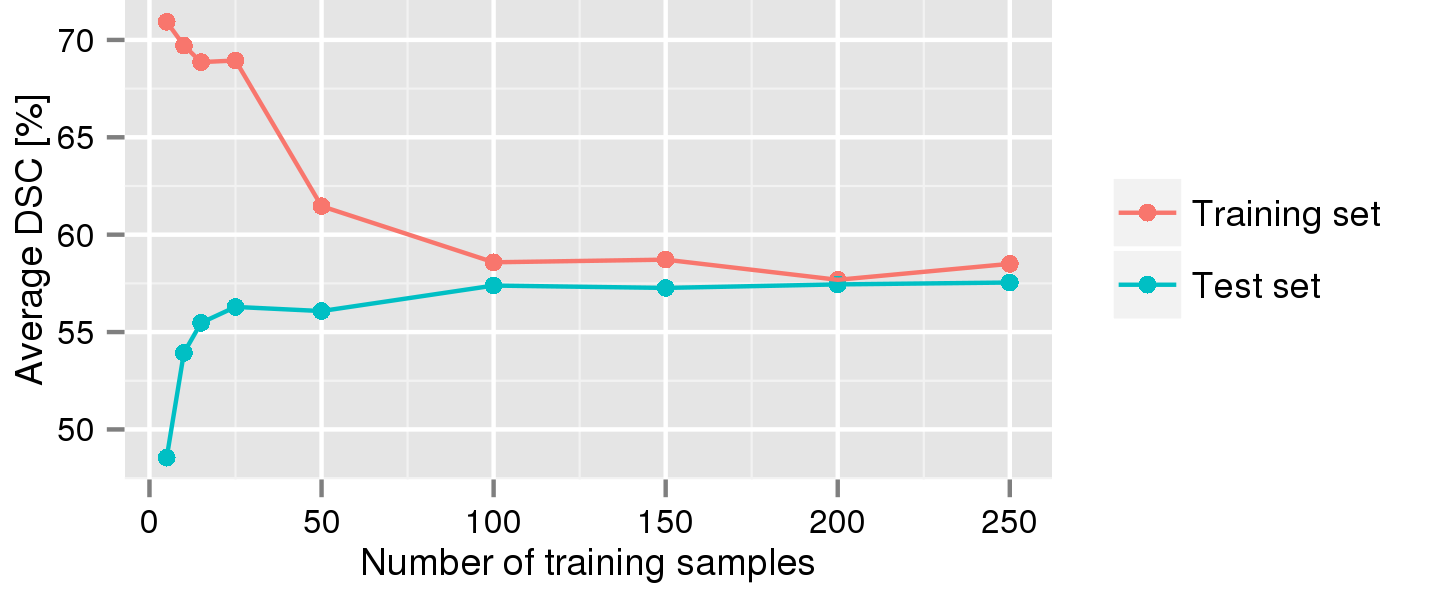
\includegraphics[width=0.78\textwidth]{figures/train_count}

\caption{Comparison of DSC scores calculated on the training and test sets for
varying numbers of training samples. At around 100 samples, the model becomes
stable in terms of test performance and the small difference between training
and test DSCs, indicating that overfitting of the training data no longer
occurs.}
\label{fig:bioms}
\end{figure}

\end{comment}
